\documentclass[11pt]{article}
%Gummi|065|=)
\title{\textbf{Algorithms in Julia}}
\author{James Schloss}
\date{}

\usepackage{graphicx}
\usepackage{hyperref}
\usepackage{listings}
\usepackage{color}

\definecolor{dkgreen}{rgb}{0,0.6,0}
\definecolor{gray}{rgb}{0.5,0.5,0.5}
\definecolor{mauve}{rgb}{0.58,0,0.82}

\lstset{frame=tb,
  language=python,
  aboveskip=3mm,
  belowskip=3mm,
  showstringspaces=false,
  columns=flexible,
  basicstyle={\small\ttfamily},
  numbers=none,
  numberstyle=\tiny\color{gray},
  keywordstyle=\color{blue},
  commentstyle=\color{dkgreen},
  stringstyle=\color{mauve},
  breaklines=true,
  breakatwhitespace=true,
  tabsize=3
}


\begin{document}
\maketitle
In this document, we have descriptions of the following algorithms:
\begin{itemize}
\item Monte Carlo
\item Convolution / Edge Detection for simple images
\item Split-Operator method for solving the Schrodinger Equation
\item Julia Fractal
\item Force Integration
\item Barnes-Hut (N-body galaxy simulation)
\item FFT
\end{itemize}

All algorithms can be found in the examples directory of the \texttt{skillpill-julia} repository on github

\newpage
\section*{Monte Carlo}

There are many different methods that all work under the basic Monte Carlo principle of using random numbers to integrate systems.
For the sake of time and brevity, please refer to the following link for more information on Monte Carlo Integration: \url{http://leios.github.io/Batman_Montecarlo/}. From there, modify the provided code to work in Julia and to integrate $x^2$ where $-3 < x < 3$.

My function reads in a total range in x along with the number of points to sample. Try to match (or beat) the following benchmark:

\begin{lstlisting}
julia> @benchmark monte_carlo(6.0, 100000)
BenchmarkTools.Trial: 
  memory estimate:  0 bytes
  allocs estimate:  0
  --------------
  minimum time:     573.931 μs (0.00% GC)
  median time:      578.105 μs (0.00% GC)
  mean time:        596.870 μs (0.00% GC)
  maximum time:     1.125 ms (0.00% GC)
  --------------
  samples:          8326
  evals/sample:     1

\end{lstlisting}

\newpage
\section*{Edge Detection}
This is more about technical implementation than algorithms; however, Canny Edge Detection is a staple algorithm used in many areas -- most importantly image analysis. It is basically composed of 5 steps:
\begin{enumerate}
\item Apply Gaussian filter to smooth the image in order to remove the noise
\item Find the intensity gradients of the image
\item Apply non-maximum suppression to get rid of spurious response to edge detection
\item Apply double threshold to determine potential edges
\item Track edge by hysteresis: Finalize the detection of edges by suppressing all the other edges that are weak and not connected to strong edges.
\end{enumerate}

For the most part, this edge detection can be done relatively simply with the following code:

\begin{lstlisting}
# First, we need to use the appropriate packages
using Images  # All filtering and image stuff
using ImageView # imshow for showing images, run in REPL
using TestImages # Standart example images in julia

# simple implementation of canny edge detection using in-built Julia functions
function simple_edge_detection()
    img = testimage("fabio_color_256")
    img_edge = canny(img)
    save(string("fabio_edges.png"), img_edge)
end

simple_edge_detection()

\end{lstlisting}

However, that doesn't really show the \textbf{power} of Julia. Perform each of the 5 above steps without using the \texttt{canny} function.


\newpage
\section*{Split-Operator Method}
The Split-Operator Method is a psuedo-spectral algorithm that is important for many areas of physics, including quantum mechanics, where it is used to solve the Schr\"odinger equation,

$$
i \hbar \frac{\partial \Psi(\mathbf{r}, t)}{\partial t} = \left[\frac{-\hbar^2}{2m} \nabla^2 + V(\mathbf{r},t) \right] \Psi(\mathbf{r},t)
$$

To solve this equation, we basically split the time evolution operator ($\hat U = e^{-i \hat H t / \hbar}$) into 2 via the Baker-Campbell-Hausdorff relation:
$$\hat U_k = e^{-\mathbf{\hat p}^2 t / 2} \quad \hat U_V = e^{-V_0(\mathbf{\hat r})t/2}$$

From here, the method simply involves initializing the wavefunction and then multiplying it by half of $\hat U_V$ before flipping to momentum space via a FFT and multiplying it by all of $\hat U_k$ and then flipping back to real space with an inverse FFT and multiplying by the other half of $\hat U_V$, as shown in figure \ref{fig:split-op}

\begin{figure}
\begin{center}
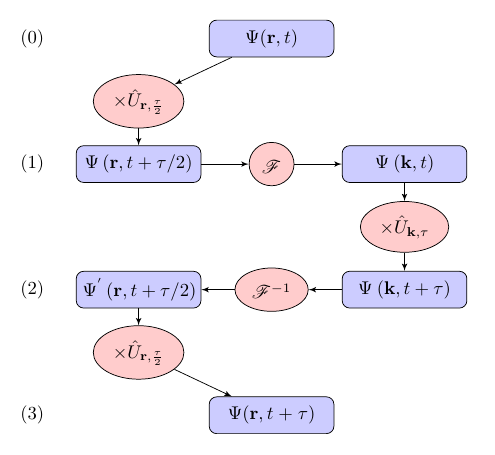
\includegraphics[width = 0.5\textwidth]{split-op.png}
\end{center}
\caption{A single step in the split-op method as described in the description}
\label{fig:split-op}
\end{figure}

\newpage
\section*{Julia Fractal}
Fractals are cool. They are structures that continually repeat themselves no matter how far you zoom in. Because we are using Julia, the obvious fractal to work with is the Julia Fractal. Full implementation details in Python can be found here: \url{https://batchloaf.wordpress.com/2013/02/10/creating-julia-set-images-in-python/}. Basically, all we need to do is iteratively solve the following formula:
$$z_{n+1} = z_n^2 + c$$
Every iteration, we reduce pixel color by 5 and recalculate z until either the pixel color is 0 or $|z|$ exceeds a provided cutoff value (somewhat arbitrary). It should be noted here that $c$ is entirely complex and that the value dratically changes the output fractal.

Create the following: 
\begin{enumerate}
\item A function that sweeps through different $c$ values and outputs an image for each value
\item A function that zooms into a fractal of $c=1.0$ to see it's self-similar nature
\end{enumerate}

If you want to, you can even combine the images into a gif by using some additional tool (like ffmpeg)
\begin{figure}
\begin{center}
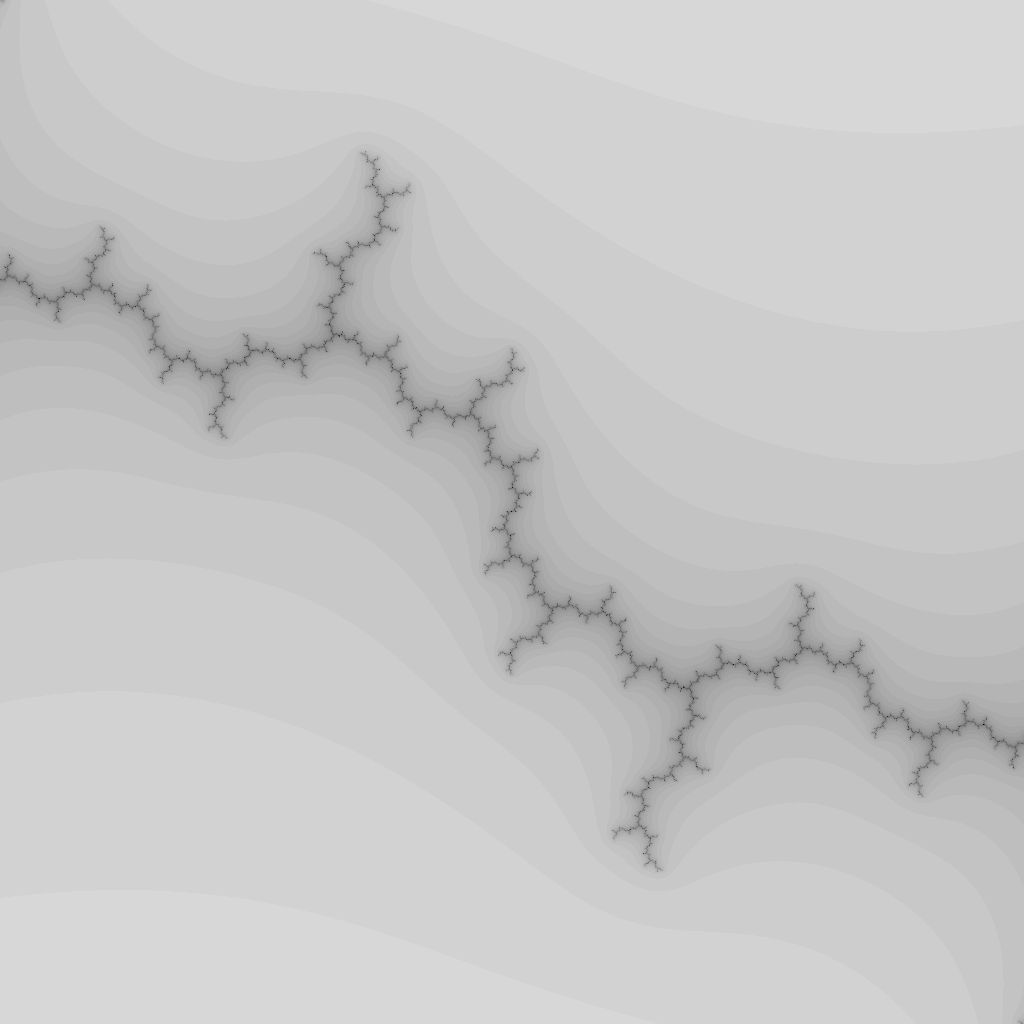
\includegraphics[width=0.45\textwidth]{fractal_zoom00030.png}
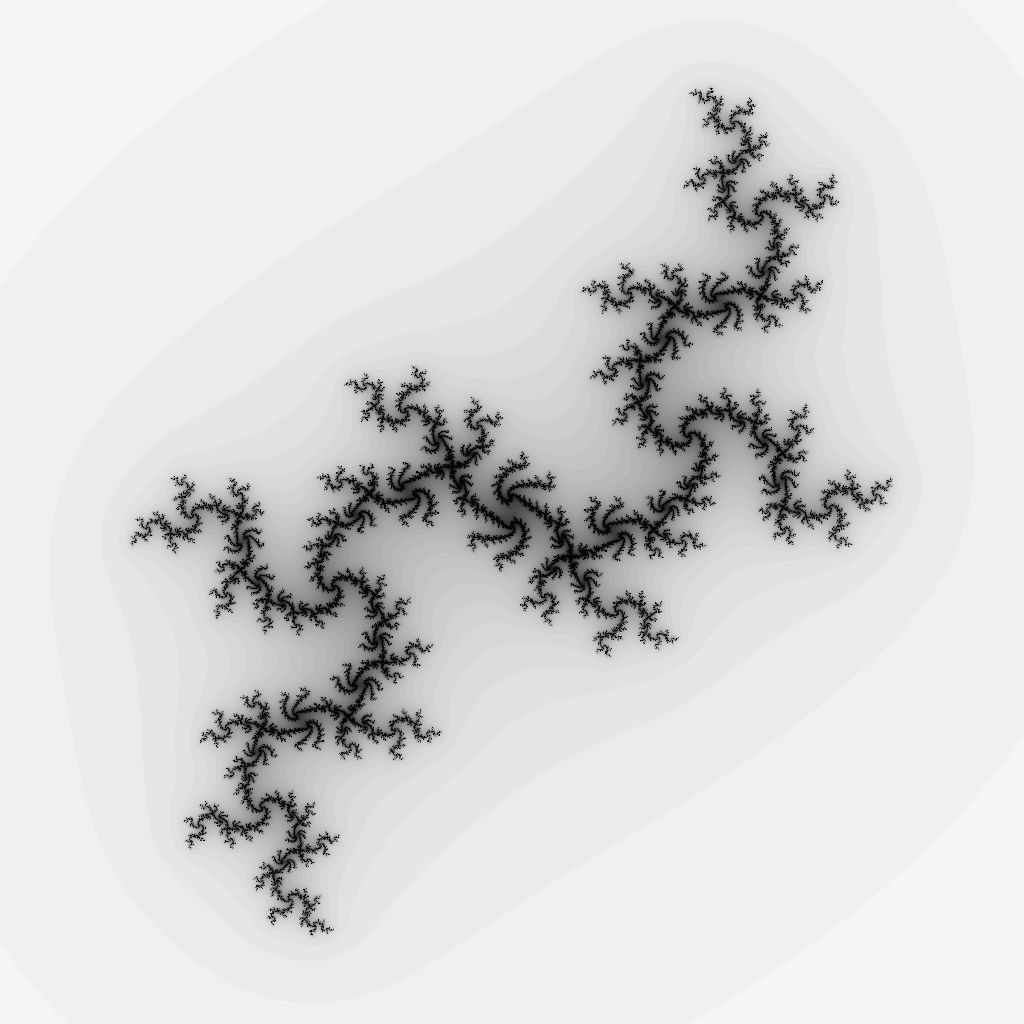
\includegraphics[width=0.45\textwidth]{c_scan00030.png}
\end{center}
\end{figure}

\newpage
\section*{Force Integration}
Integrating forces is a staple of any physics engine and most physics simulations. Though there are many different algorithms, here we focus on the Verlet algorithm (because it's conceptually simple); however, if you want to implement Runge-Kutta4 (or whatever), feel free to do so!

First, let's start with the Taylor Series Expansion:

$$x = x_0 + v_0 t + \frac{1}{2}at^2 + \ldots$$

If we are looking for $x(t + \Delta t)$, we can start by looking at the timesteps immediately before it:
$$x(t+\Delta t) = x(t) + v \cdot \Delta t + \frac{1}{2} a\cdot\Delta t^2$$
$$x(t-\Delta t) = x(t) - v \cdot \Delta t + \frac{1}{2} a\cdot\Delta t^2$$

Adding these together and solving for $x(t + \Delta t)$, we get:

$$x(t + \Delta t) = 2x(t) - x(t - \Delta t) + a \Delta t^2$$

This means we can solve for any object's new position if we know it's acceleration and where it's been! Of course, if we need the velocity (possibly to solve for the acceleration of a damped system), we can find it with:

$$v(t) = \frac{x(t + \Delta t) - x(t - \Delta t)}{2\Delta t}$$

Now, let's integrate some forces! Start with a ball at a height of 5m. How long does it take to hit the ground? Also, plot it's trajectory with time.

\newpage
\section*{Barnes-Hut}
Using the previous section on force integration, we know that all we really need for an N-body gravity simulator is a method to calculate the acceleration of an object in space. In principle, this is straightforward: We just add up all the particles and calculate

$$a = \frac{GMm}{r^2}$$

In practice, this means that we have an $O(n^2)$ problem on our hands! That said, we can take our N-body simulation and speed it up drastically with the help of a rather famous data structure known as an octree (or quadtree in 2d).

These data structures are straightforward. The root node is the entire simulation box, it's children are the octants of that box. Each octant has 8 octchildren, and we keep splitting up the simulation until every particle has it's own box. At this point, it's not obvious how this speed anything up; however, each box has a Center of Mass equal to all the elements on the inside of it. If our objects are sufficiently far away from each other, we can take a larger parent box instead of a smaller child box. This cuts computational time tremendously!

In particular, the cutoff value is defined as $\theta = s/d$ where $s$ is the width of the region represented by the internal node and $d$ is the distance between the body and it's Center of Mass. By playing with $\theta$, we can have either a fast, inaccurate simulation or a slow, accurate one. The trick is finding the happy-medium between the two!

\newpage
\section*{FFT}
FFT's are everywhere nowadays. In fact, we used it previously in this document when talking about the Split-Operator method. For the most part, FFT's use an implementation of the Cooley-Tukey algorithm, which basically involves recursively dividing the array we wish to transorm into even and odd components and solving them with a slow Discrete Fourier Transform (DFT) when we get below a certain number of elements. 

By solving our system recursively, we can take an $O(n^2)$ process to $(n\log n)$, which is hughe savings! Full implementation details can be found here: \url{https://leios.gitbooks.io/algorithm-archive/content/chapters/computational_mathematics/cooley_tukey.html} (you might need to refresh the page to get the formulas to work)

\end{document}
